\section{CALCULOS} 
\subsection{AGREGAR UNA COLUMNA CALCULADA}

\begin{itemize}

\item 1. En Power BI Desktop, haga clic en Datos en el panel de vistas en el lado izquierdo.
añadir el control al reporte.
\item 2. En el panel Campos, haga clic en DimCustomer.
\item 3. En la cinta de Modelado, en el grupo Cálculos, haga clic en Nueva columna.\\
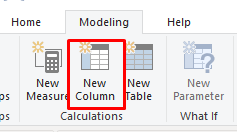
\includegraphics[scale=0.5]{./Imagenes/image015}
\item 4. En la barra de fórmulas, resalte Columna = y escriba: \\
IncomeStatus = IF (DimCustomer[YearlyIncome] < 25000, "Lower Income",\\
IF (AND(DimCustomer[YearlyIncome] >= 25000, DimCustomer[YearlyIncome] < 60000),\\
"Middle Income",\\
IF (AND(DimCustomer[YearlyIncome] >= 60000, DimCustomer[YearlyIncome] < 100000),\\
"Higher Income",\\
IF (DimCustomer[YearlyIncome] >= 100000, "Very High Income", "Other")))) \\

\item 5. Presione Enter. \\
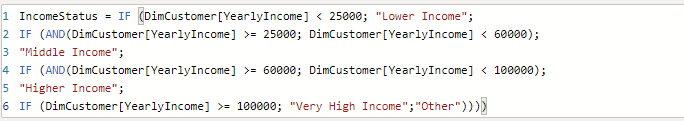
\includegraphics[scale=0.5]{./Imagenes/image016}
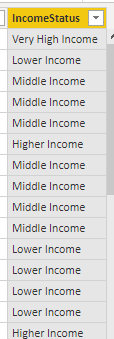
\includegraphics[scale=0.5]{./Imagenes/image017}

\item 6. En la cinta de Modelado, en el grupo Cálculos, haga clic en Nueva columna.
\item 7. En la barra de fórmulas, resalte Columna = y escriba: \\
DaysSinceFirstPurchase = DATEDIFF(DimCustomer[DateFirstPurchase], TODAY(), DAY) \\
\item 8. Presione Enter. \\

\includegraphics[scale=0.5]{./Imagenes/image018}
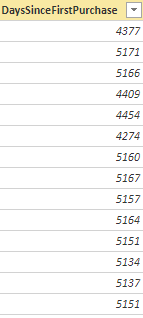
\includegraphics[scale=0.5]{./Imagenes/image019}
\item 9. En la cinta de Modelado, en el grupo Cálculos, haga clic en Nueva columna.

\item 10. En la barra de fórmulas, resalte Columna = y escriba: \\
FullName = [FirstName] [LastName] \\

\item 11. Presione Entrar. \\


\includegraphics[scale=0.5]{./Imagenes/image020}
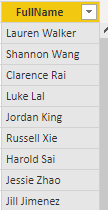
\includegraphics[scale=0.5]{./Imagenes/image021}

\item 12. En la cinta de Modelado, en el grupo Cálculos, haga clic en Nueva columna.
\item 13. En la barra de fórmulas, resalte Columna = y escriba:\\
MaleFemale = IF ([Gender] = "M", "Male", "Female")

\item14. Presione Entrar.\\
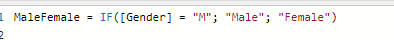
\includegraphics[scale=0.5]{./Imagenes/image022}
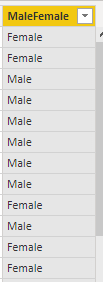
\includegraphics[scale=0.5]{./Imagenes/image023}

\item 15. En la cinta de Modelado, en el grupo Cálculos, haga clic en Nueva columna.

\item 16. En la barra de fórmulas, resalte Columna = y escriba:\\
Relationship = IF([MaritalStatus] = "M", "Married", "Single")\\
\item 17. Presione Entrar. \\
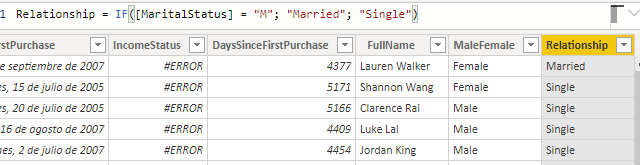
\includegraphics[scale=0.5]{./Imagenes/image024}
\item 18. En el panel Campos, haga clic en DimProductSubcategory.

\item 19. En la cinta de Modelado, en el grupo Cálculos, haga clic en Nueva columna.

\item 20. En la barra de fórmulas, resalte Columna = y escriba:\\
MainCategory = RELATED (DimProductCategory [CategoryName])
\\
\item 21. Presione Entrar.\\
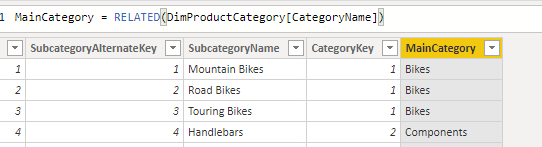
\includegraphics[scale=0.5]{./Imagenes/image025}
\item 23. En la cinta de Modelado, en el grupo Cálculos, haga clic en Nueva columna.
\item 24. En la barra de fórmulas, resalte Columna = y escriba:\\
PromotionLengthDays = DATEDIFF (DimPromotion [StartDate], DimPromotion [EndDate], DAY)\\

\item 25. Presione Entrar.\\
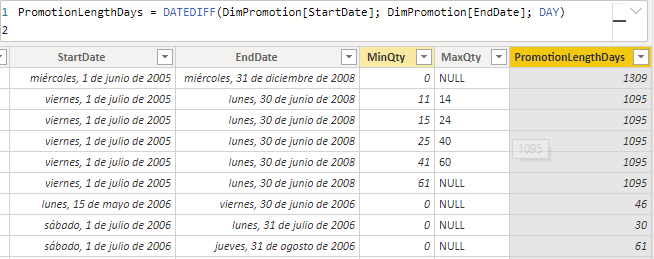
\includegraphics[scale=0.5]{./Imagenes/image026}
\item 26. En el panel Campos, haga clic en FactInternetSales.
\item 27. En la cinta de Modelado, en el grupo Cálculos, haga clic en Nueva columna.
\item 28. En la barra de fórmulas, resalte Columna = y escriba:\\
Profit = CURRENCY(FactInternetSales[UnitPrice] - \\
FactInternetSales[ProductStandardCost])\\
\item 29. Pressionar Enter.\\
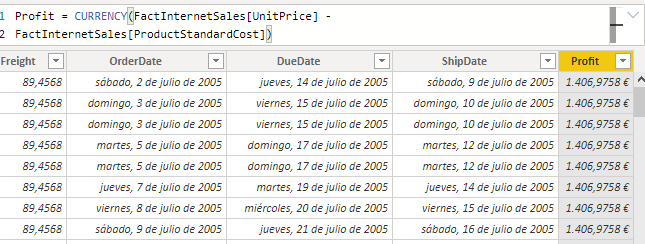
\includegraphics[scale=0.5]{./Imagenes/image027}
\item 30. Cerrar Power BI Desktop, salvando cualquier cambio. \\
LINK: https://app.powerbi.com/groups/me/reports/9800665a-badd-4100-a74f-4fea5114c745/ReportSection

\end{itemize}